\subsection{Modelo de Holt}
\begin{figure*}
    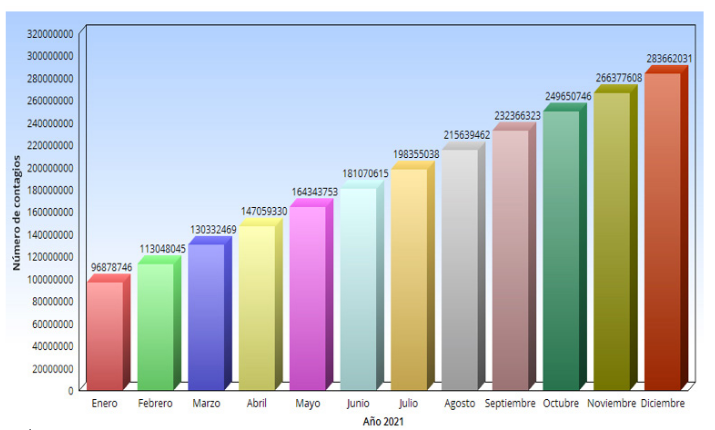
\includegraphics[width=\textwidth]{holtz.png}
    \caption{Predicción de número de contagios a nivel mundial utilizando el modelo de Holtz. Fuente: \cite{diazpinzon_2020}}
    \label{holtz}
\end{figure*}

El modelo de Holt, similar al modelo de Gompertz, es un modelo conocido por ser una modificación al modelo de suavización exponencial simple, a través de una constante de suavización $\delta$. Este modelo es expresado matemáticamente por la siguiente expresión:

\begin{equation*}
    Y_t = L_t + p T_t
\end{equation*}

Donde:
\begin{itemize}
    \item $Y_t$: valor pronosticado para el periodo $t$.
    \item $L$: valor estimado para el periodo $t$.
    \item $T_t$: valor de la tendencia para el periodo $t$.
    \item $p$: valor a pronosticar en el futuro.
\end{itemize}

Esta variable $L$ es definible bajo la siguiente equación:

\begin{equation*}
    L_t = \alpha Y_{t-1} + (1-\alpha)(L_{t-1} + T_{t-1})
\end{equation*}

Donde:
\begin{itemize}
    \item $\alpha$: constante de suavización, cuyo valor se encuentra entre 0 y 1.
    \item $Y_{t-1}$: valor de la variable pronostricada en el periodo anterior.
\end{itemize}

A su vez, la variable $T$ es definida de la siguiente manera:
\begin{equation*}
    T_t = \beta (L_t - L_{t-1}) + T_{t-1} (1 - \beta)
\end{equation*}

Donde:
\begin{itemize}
    \item $\beta$: es una constante de suavización por modificación de la tendencia, también restringido entre 0 y 1.
\end{itemize}

Este modelo fue utilizado por el autor Díaz Pinzón, J. E., en su documento "Predicción del COVID-19 a nivel mundial para el año 2021"\cite{diazpinzon_2020}. La predicción resultante puede ser encontrada en la figura \ref{holtz}